The input voltage is set to $u_e = A_u sin(2\pi f_c t)$, where $A_u = 5 \ V$ and $f_c = 20 \ Hz$.
Then the nonlinear system implemented in P2 is simulated to get the states responses. For more clarity, the time domain responses were plotted from 0 to 2s. Moreover, the system is not stabilised at the beginning of the simulation, so it was decided to remove the first second for the spectral analysis. To visualise the signals in the frequency domain, we used the \textit{$power\_spectral\_density$} function given in the assignment \cite{assign} with $F_s = \frac{1}{STEP\_SIZE} = 10 \ kHz$. The function output gives the power spectral density $P_{xx}$ in [$Amplitude^2$/Hz]. In order to convert it in [dB/Hz], we use: 
\begin{equation*}
P_{dB} = 10log_{10}(P_{xx})
\end{equation*} 

\begin{figure}[H]
 \centering 
 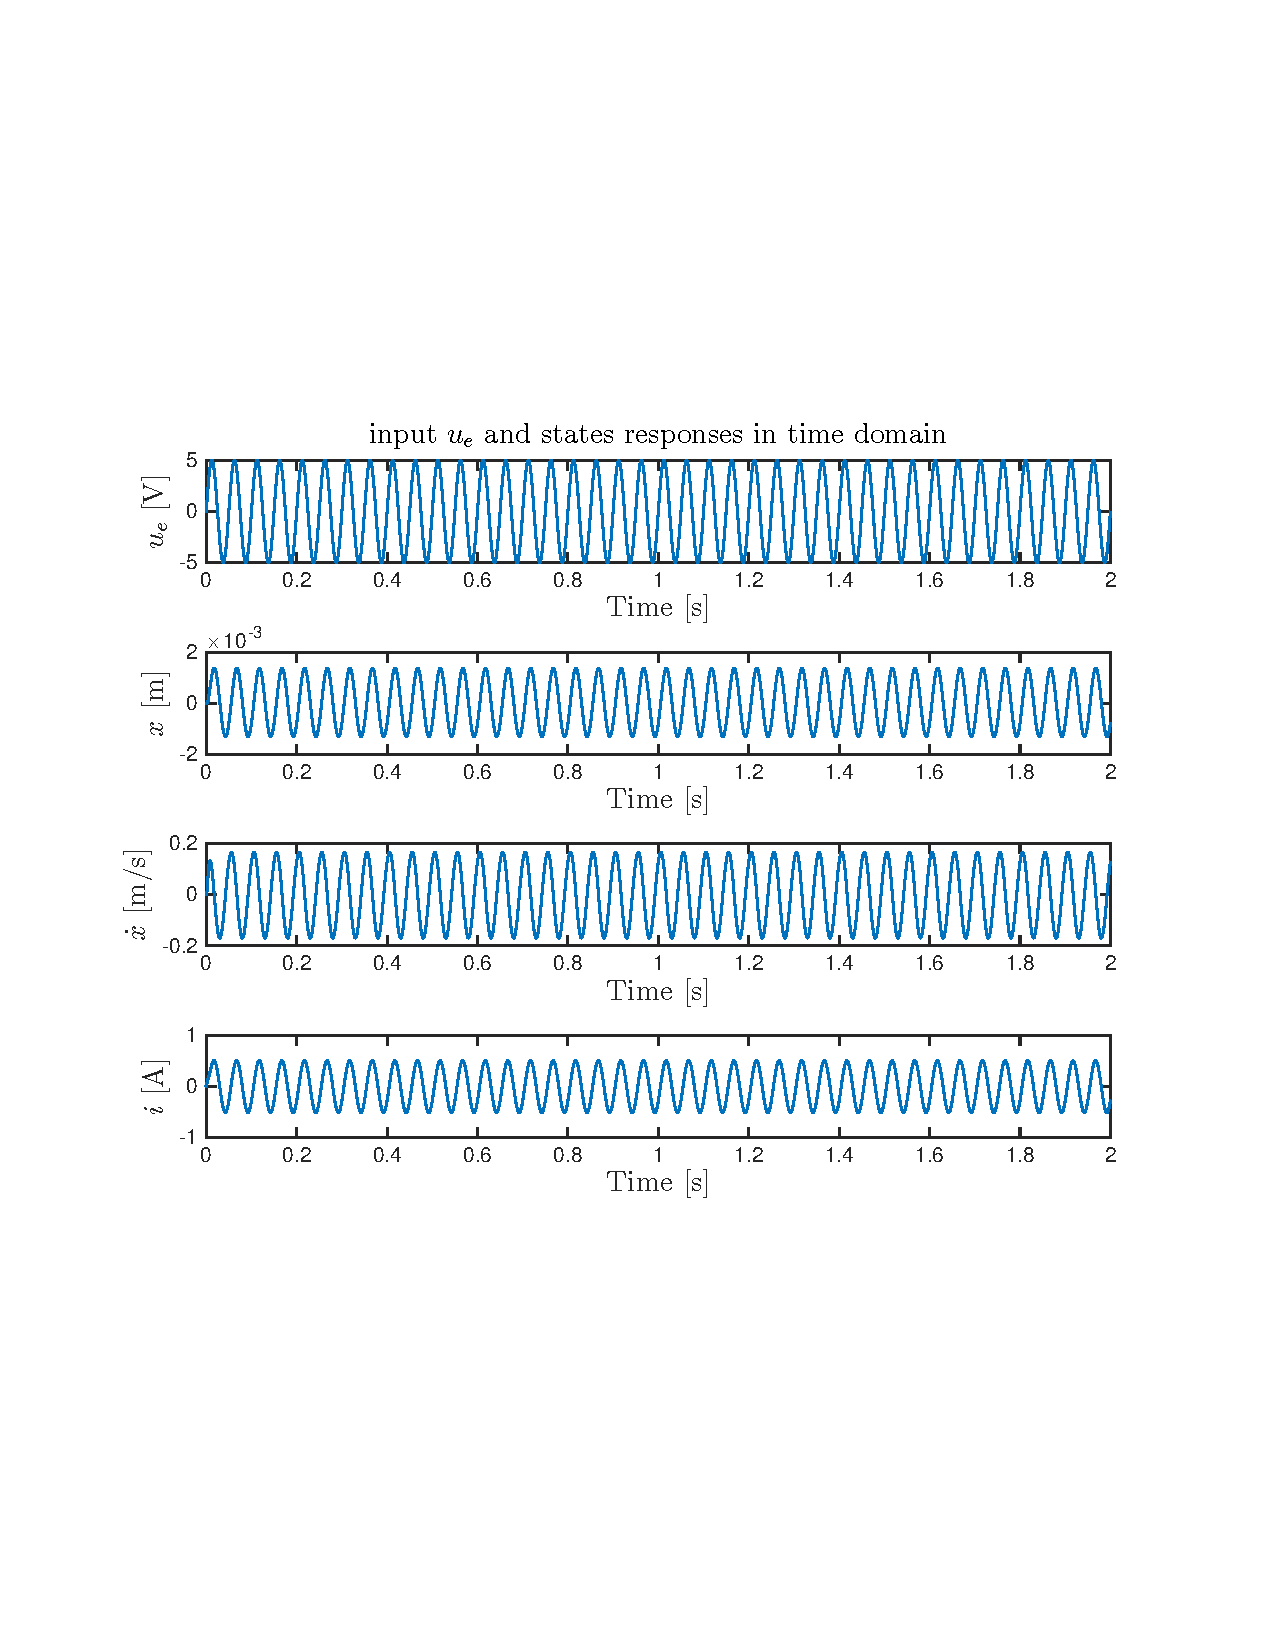
\includegraphics[trim=2cm 7cm 2cm 7cm, clip=true, totalheight=0.35\textheight, angle=0]{figures/P3timeDomain.pdf}
 \caption{Nonlinear Model: input $u_e$ and the states responses in the time domain}
 \label{fig:NLMt}
\end{figure}

\begin{figure}[H]
 \centering 
 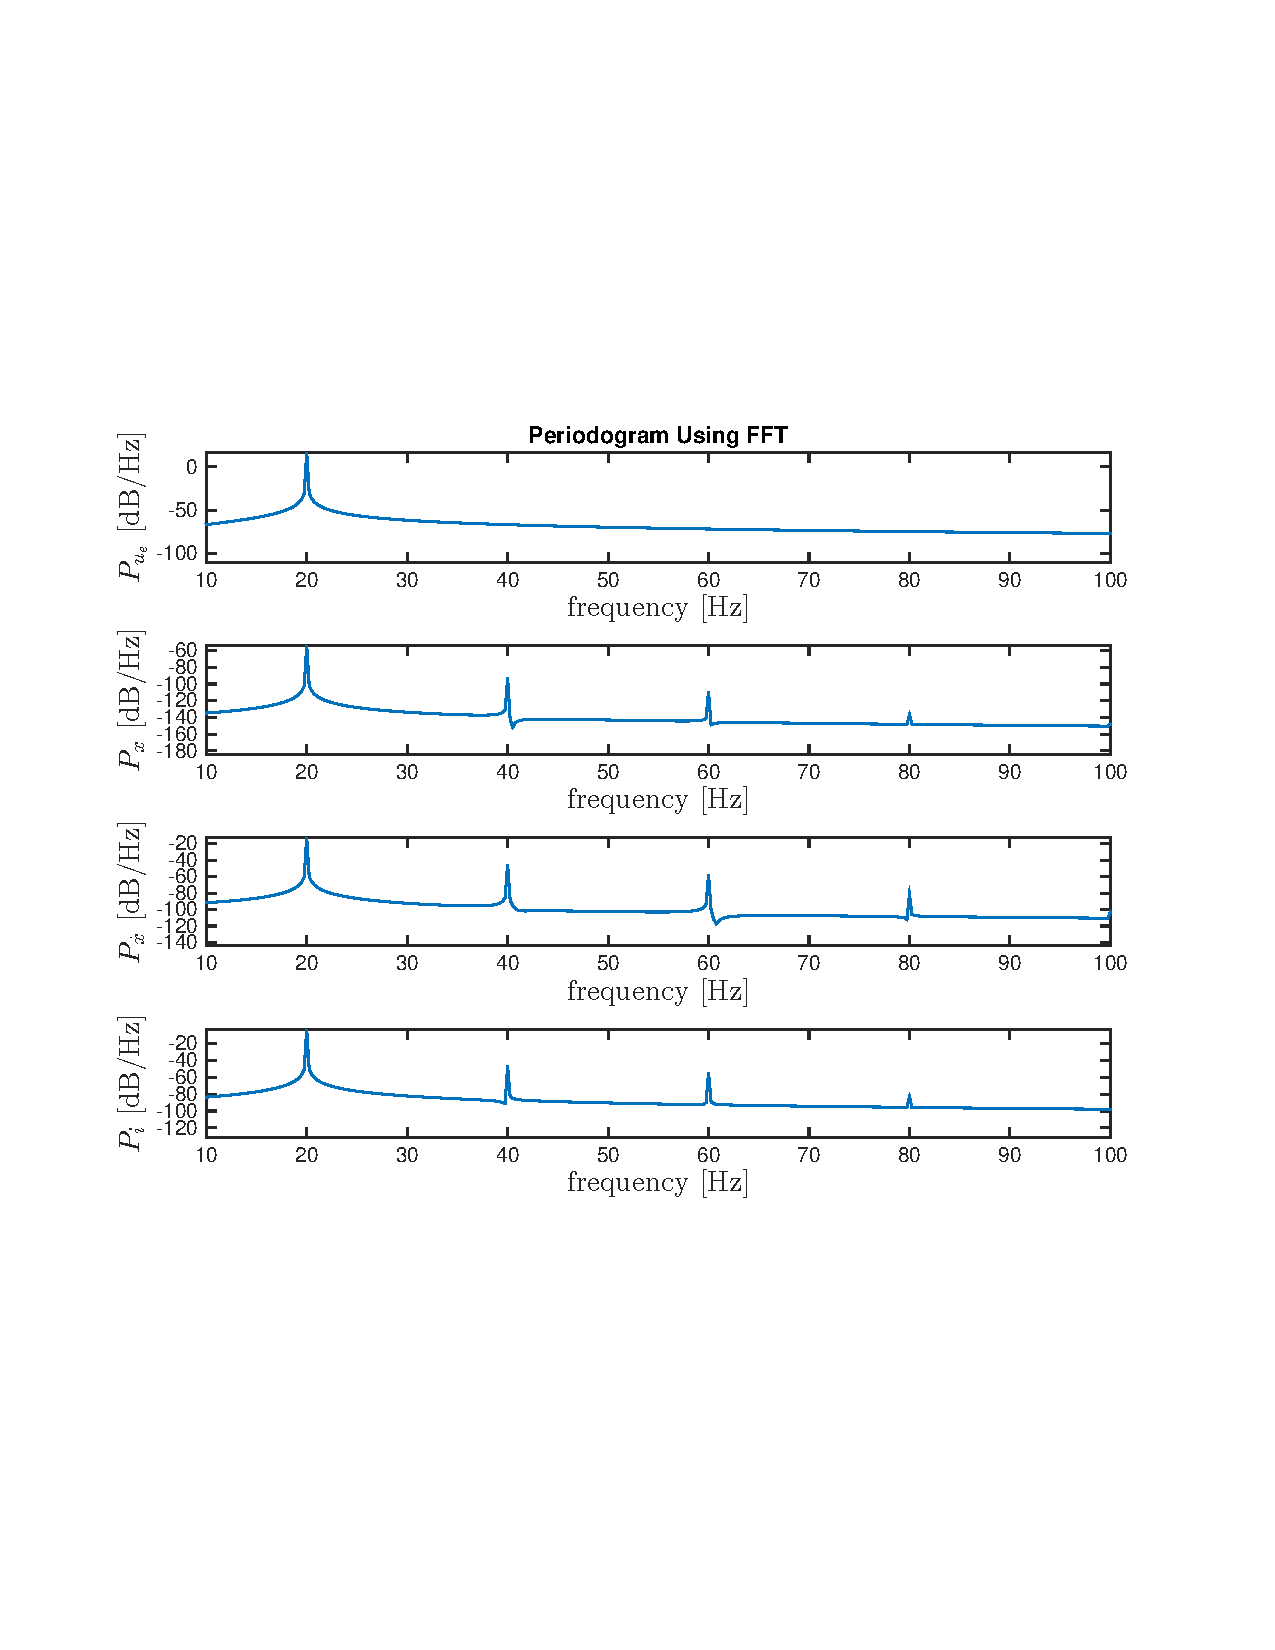
\includegraphics[trim=2cm 7cm 2cm 7cm, clip=true, totalheight=0.35\textheight, angle=0]{figures/P3frequencyDomain.pdf}
 \caption{Nonlinear Model: input $u_e$ and the states responses in the frequency domain}
 \label{fig:NLMf}
\end{figure}

In the time domain (see figure \ref{fig:NLMt}), we notice that the states responses are sinusoidal, with constant amplitudes. The system looks stable. Moreover, the frequency of the states seems similar to the frequency of the input signal, with slight variations. The explanation for these changes is given in the frequency domain, figure \ref{fig:NLMf}, where we can see several more spikes at the frequencies $f_n = nf_c$, smaller than the fundamental one at $f_c = 20 \ Hz$. The presence of other harmonics in the states responses, which are not in the input, shows the effects of the nonlinearity of the system. It may be due to the fact that the voice coil displacement is limited: when it goes too far, the spider prevents it from leaving the magnetic field, which can cause the harmonic distortion. 